\documentclass[11pt,a4paper]{article}

\usepackage[utf8]{inputenc}
\usepackage[T1]{fontenc}
\usepackage[margin=2.4cm]{geometry}
\usepackage{amsmath}
\usepackage{booktabs}
\usepackage{longtable}
\usepackage{graphicx}
\usepackage[hidelinks]{hyperref}

\setlength{\parskip}{3pt}
\setlength{\emergencystretch}{2em}
\newcommand{\hx}[2]{\texttt{#1}\allowbreak\texttt{#2}}

\title{Entity-Centric High-Recall Retrieval for Scientific ``Which Methods'' Questions:\\
A Development-Only Redesign (V2, Second Iteration)}
\author{Experiment: \texttt{entity\_centric\_high\_recall\_v2} \\
Working tree: \texttt{clean\_tshc\_v2} \quad Primary system: \texttt{A7} \quad Label: DEVELOPMENT}
\date{2 October 2026}

\begin{document}
\maketitle

\begin{abstract}
This report documents a frozen, development-only redesign of an entity retrieval pipeline over a
materials-informatics knowledge graph snapshot. The prior V1 system and a first V2 attempt both failed at
the \emph{candidate-admission} stage: the correct answer entities were usually absent from the top of the
candidate list, so no reranking strategy could repair the outcome. The redesign therefore targets admission
first: canonical entity grouping with graph-provided aliases and type families, a separately indexed
evidence store derived from inferred schema roles, \emph{six} retrieval lists (dense over the raw question,
dense over a structured view, BM25, safe name matching, evidence-dense, and bounded graph expansion --- five
channel families if the two dense views are counted as one), a deterministic union, and reciprocal rank
fusion. A genuine MS MARCO relevance cross-encoder reranks a fixed prefix, and a pinned local
natural-language-inference model is used as an explicitly uncalibrated \emph{requirement-verification
proxy} with four-status semantics over a stable top-20 tiering. Every entity channel applies the same
\textbf{hard} answer-family type filter; there is no soft type prior in this pipeline.
The predeclared hypothesis is \textbf{partly supported}. Candidate recall rose decisively: the A5 fusion arm
admits 37/49 directly mapped target occurrences by depth 100, 44/49 by depth 500, and 46/49 in the full
union, against 3/49 at depth 100 for the previous V2 high-recall arms. Final ranking did not follow
proportionally. The declared primary system A7 recovers 10 of 63 target occurrences at top-10 (15.87\,\%),
against 3/63 for the previous V2's dense baseline and 2/63 for its relevance arm, but a predeclared
smaller-pool control, \texttt{A6\_100}, reaches 12/63; mean reciprocal rank is \emph{higher} for the simple
round-robin union A4 (0.2013) than for A5 (0.1554), A6 (0.1480) or A7 (0.1516). Among the 44 target
occurrences admitted to the 500-deep reranking pool, 18 moved up and 26 moved down, with the conditional
median rank moving from 39 to 50.5. High recall did not deliver proportional ranking quality, and the larger
reranking pools were worse on top-10 recovery here. All numbers are development diagnostics from frozen
artifacts of a single seeded run; no held-out, variance or inferential-superiority claim is made.
\end{abstract}

\tableofcontents

\section{Motivation}

\subsection{What V1 and the first V2 established}

The task is a small set of expert-authored scientific questions of the form ``Which methods (by Feb 2026)
are best suited for \ldots{}'' and ``What are the leading \ldots{}'', each annotated with one or more target
answer entities. The retrieval corpus is a knowledge graph snapshot containing typed nodes
(\texttt{method}, \texttt{technique}, \texttt{component}, \texttt{cited\_work}, \texttt{dataset},
\texttt{metric}, \texttt{article}) and typed relations.

V1 used a single dense bi-encoder over a bounded textual rendering of each graph node. Its failure mode was
not subtle ranking error but outright absence: in the current matched re-run, the V1-like control A0 admits
only 6 of 49 directly mapped target occurrences anywhere in a 500-candidate list, and recovers 0 at top-10.
The first V2 iteration, archived under \texttt{archive/flat\_20261001}, attempted richer scoring without
fixing admission; its high-recall arms (\texttt{V2-B}, \texttt{V2-C}) admitted only 3 of 49 mapped
occurrences at depth 100 and recovered 1 and 2 occurrences respectively at top-10, with MRR 0.0168 and
0.0566, while its own dense baseline arm recovered 3.

Two lessons drive this redesign. First, \emph{admission constrains everything downstream}: each later
component is conditioned on a pool it cannot extend, so recall at realistic depths must be measured and
reported before any reranking claim. Second, \emph{rank statistics must be explicit about misses}. The
archived arms' rank means were computed over the full corpus, where every target necessarily has some rank
and the miss count is zero by construction. Those figures are valid under that protocol; they are simply a
different quantity from the conditional means over a truncated candidate list reported here, and the two are
not comparable without also reporting misses.

\subsection{Development-only status}

The benchmark questions and their gold annotations were already inspected by the author during V1
development, and that exposure motivated this redesign. Separating prediction from evaluation at execution
time (Section~\ref{sec:leak}) removes \emph{execution-time} leakage: the predictor cannot read gold files,
historical outputs, reports, notes, or the evaluator. It does not and cannot remove the fact that the
benchmark had already influenced the design and the request. No claim is made here about the precise extent
of any design-time exposure beyond that. Consequently:

\begin{itemize}
\item every number in this report is a \textbf{development diagnostic};
\item no claim of inferential or statistical superiority over V1, prior V2, or any external system is made
or justified;
\item with 14 scored questions and 63 target occurrences, differences of one or two occurrences are at the
resolution of the measurement and are reported as observations, not as effects.
\end{itemize}

\subsection{Predeclared hypothesis}

\textbf{Hypothesis.} Replacing single-channel dense node retrieval with entity-centric canonical grouping,
a separately indexed evidence store, multi-channel deterministic union and rank fusion will (H1) raise
candidate recall of directly mapped target occurrences at operationally useful depths by a large margin, and
(H2) that this improved admission, combined with a genuine relevance cross-encoder and a
requirement-verification reranking stage, will translate into materially better top-10 identity recovery.

\textbf{Verdict: partly supported.} H1 is supported \emph{by the observed development evidence} on candidate
recall (Section~\ref{sec:recall}); the measurement is a single run on a design-exposed question set, so the
support is for the recall claim as measured, not an unqualified general result. H2 is mixed. Top-10 recovery
rose from 3/63 (previous V2 dense baseline) and 2/63 (previous V2 relevance arm) to 10/63 for A7, but that
overall comparison involves a redesigned index, new channels and new fusion, and therefore does not isolate
the contribution of the cross-encoder. Within the matched new run the incremental reranking picture is
mixed: top-10 hits move 6 (A5) $\to$ 9 (A6) $\to$ 10 (A7) while MRR moves 0.1554 $\to$ 0.1480 $\to$ 0.1516,
and a predeclared smaller-pool control beats the declared primary on top-10.

\section{Data and time semantics}

All current questions are evaluated against the frozen \textbf{2026 snapshot}. The index built for that
snapshot contains 2978 canonical entities, 4274 evidence items, 10241 entity--evidence links and 6368
inferred role arcs, with 0 rejected edges and 2508 entities possessing \emph{no} candidate-specific evidence
(Table~\ref{tab:index}). These are \textbf{index object counts} --- entities, evidence items, links, arcs
--- and must not be read as target-occurrence counts; the occurrence-based counts used for scoring are
defined in Section~\ref{sec:metrics}.

The 2508 figure (84.2\,\% of entities) bounds what the evidence-dependent machinery can do: for those
entities requirement verification has no eligible candidate-specific premise. Article or structural
context may still provide evidence-retrieval links or cross-encoder context; otherwise the card contains
identity alone. They remain retrievable through the two dense channels, which score bounded renderings of
their member nodes, and through BM25, whose per-entity lexical document always contains the entity's names
and graph aliases (Section~\ref{sec:lex}).

\begin{table}[htbp]
\centering
\caption{Frozen 2026 index statistics. These are index object counts, not scored occurrences.}
\label{tab:index}
\begin{tabular}{lr}
\toprule
Quantity & Value \\
\midrule
Canonical entities & 2978 \\
Evidence items & 4274 \\
Entity--evidence links & 10241 \\
Inferred role arcs & 6368 \\
Rejected edges & 0 \\
Entities without candidate-specific evidence & 2508 \\
\bottomrule
\end{tabular}
\end{table}

Time semantics are deliberately conservative:

\begin{itemize}
\item \texttt{first\_seen\_year} defines \emph{publication visibility within this graph}: an entity is
visible to a query with cutoff $y$ only if $\texttt{first\_seen\_year} \le y$. It is the first year the
graph records the entity, which is not a guarantee of the actual date of discovery or first use.
\item \texttt{last\_seen\_year} is \textbf{not} an expiry date. An entity last observed in 2021 is not
removed from a 2026 query. Only its \emph{undated aliases} are affected: because alias annotations carry no
individual dates, aliases contributed by a member node are suppressed when that node's last observation
\textbf{exceeds} the snapshot cutoff being constructed. The rule therefore only bites when the parser
derives a cutoff earlier than the node's last observation; for a 2026 query over the 2026 snapshot nothing
is suppressed by it.
\item When the parser derives an earlier year cutoff, an edge must pass \emph{both} the edge-year check and
the asserting-article-year check; an edge whose own year is admissible but whose asserting article postdates
the cutoff is rejected.
\item Month precision cannot be recovered from year-only evidence. Questions phrased ``by Feb 2026'' are
therefore answered with year granularity. This is an unavoidable approximation, not a modelled constraint.
\end{itemize}

\section{Canonical entities, aliases and type families}

Surface normalization applies, in order: Unicode NFKC, casefolding, whitespace collapse, and
typographic-hyphen normalization to ASCII hyphen. All other punctuation is \emph{preserved}. Writing
$\nu(\cdot)$ for this normalizer, two member nodes $m_i, m_j$ merge into one canonical entity only if

\begin{equation}
\nu(\text{name}(m_i)) = \nu(\text{name}(m_j))
\quad\wedge\quad
\mathcal{F}(\text{type}(m_i)) = \mathcal{F}(\text{type}(m_j)),
\label{eq:merge}
\end{equation}

where $\mathcal{F}$ maps a node type to its family. The \emph{approach} family is
\texttt{method}, \texttt{technique}, \texttt{component}, and \texttt{cited\_work}; \texttt{dataset},
\texttt{metric} and \texttt{article} each form their own singleton family. Equation~\eqref{eq:merge}
requires \emph{identical} normalized strings: no fuzzy, embedding-based or abbreviation-based merging is
performed, because an inferred merge would assert an identity the graph does not.

The canonical identifier of an entity is derived from the \textbf{lowest member node ID}, never a gold label
and never a human-chosen preferred name, which keeps the identifier space independent of the annotation used
later for evaluation.

Aliases are taken from the graph only. Actual graph aliases are used as \emph{retrieval strings} --- they
enter the name channel and the BM25 lexical document --- but they never induce a merge under
Equation~\eqref{eq:merge}. An alias relation in the graph is evidence that a string refers to an entity;
string similarity between two entity names is not.

\subsection{Hard answer-family filtering}
\label{sec:hardfilter}

Answer type families map a question's extracted answer head(s) to admissible entity types:
\texttt{method}, \texttt{model}, \texttt{architecture}, \texttt{algorithm}, \texttt{tool} and
\texttt{system} map to the approach family; \texttt{technique} maps to
$(\texttt{technique}, \texttt{method}, \texttt{component})$; \texttt{benchmark} maps to
$(\texttt{dataset}, \texttt{metric})$; \texttt{dataset} and \texttt{metric} map to themselves; and
\texttt{article}/\texttt{paper} map to $(\texttt{article}, \texttt{cited\_work})$.

This filtering is \textbf{hard, and it is applied identically by every entity channel.} A single eligible
set is computed once per question as

\begin{equation}
\mathcal{A}(q) \;=\; \bigl\{E \;:\; \text{types}(E) \cap \textstyle\bigcup_{t \in \text{heads}(q)} \mathcal{F}am(t) \neq \emptyset \bigr\},
\label{eq:allowed}
\end{equation}

with the convention that an empty or unmapped head set admits everything. The two dense channels, BM25, the
name channel, the evidence channel and the graph expansion all restrict their output to $\mathcal{A}(q)$.
\textbf{There is no soft type prior anywhere in this pipeline.} The configuration file retains a legacy key
\texttt{soft\_type\_prior} $= 0.8$; it is \emph{unused} by this implementation and is reported here only so
that a reader inspecting \texttt{config.json} is not misled. Consequently \texttt{TypedRaw} is not ``A1 plus
hard filtering'': both arms are hard filtered, and \texttt{TypedRaw} isolates the \emph{raw-question dense
view alone} under that filter, while A1 takes the maximum over the raw and structured dense views under the
same filter. The only unfiltered arm is A0, which is the V1-like dense control over graph nodes.

The hard filter has a measured cost: three \texttt{EXACT} target occurrences in Q14 (\texttt{JARVIS-DFT},
\texttt{AFLOW}, \texttt{Alexandria}) are excluded (Section~\ref{sec:fail}). Q14 asks for ``datasets and
benchmarks'', whose families are $\{\texttt{dataset}, \texttt{metric}\}$; the graph nodes bearing those three
names carry node types outside that set, so Equation~\eqref{eq:allowed} removes them before any channel runs.
The honest description is therefore that these are scientific targets the question requests \emph{as}
datasets/benchmarks whose \emph{graph typing} differs from the requested families; no claim is made here
about what the graph does type them as, because that was not inspected for this report.

\section{Query representation}

The \textbf{original question is retained verbatim}, including every modifier, and it is the string used as
the relevance query for the cross-encoder. Extractive structure is strictly supplementary. A deterministic
extractive parser produces:

\begin{itemize}
\item the answer head(s) and the corresponding type families;
\item \emph{preserved pre-head scientific modifiers} --- e.g.\ ``universal'' in ``universal MLIPs'',
``twisted van der Waals'' in Q3 --- kept attached rather than stripped as stopword-like qualifiers, since in
this domain the modifier usually carries the discriminating content;
\item coordinated answer families, so that ``datasets and benchmarks'' in Q14 yields a union of admissible
families rather than an arbitrary single choice;
\item core requirements, additional requirements and exclusions, used only by the verification stage.
\end{itemize}

Two query views are scored independently: the original question $q_{\text{o}}$ and a structured rendering
$q_{\text{s}}$. A third, parsed-only view $q_{\text{p}}$ is encoded solely to drive the
\texttt{ParsedOnly} control and never enters the union. \texttt{ParsedOnly} is markedly worse than the
original-question arms (MRR 0.0843 versus 0.1666 for A1). The supportable reading is narrow: on these 14
questions, with this encoder and this rendering, replacing the raw question by the structured rendering lost
ranking quality, which is why the raw question is retained. It does not establish that extractive parsing
destroys information in general, and indeed the structured dense view recovers slightly \emph{more} mapped
occurrences than the original-question view (21 versus 19, Table~\ref{tab:channel}).

\section{Indexed evidence and role inference}

\subsection{Separate evidence encoding}

Every evidence node is encoded \emph{separately} by type: \texttt{claim}, \texttt{task}, \texttt{problem},
\texttt{technique}, \texttt{component}, \texttt{dataset}, \texttt{metric}, \texttt{article}. Each entity
links to its evidence with source IDs, relation paths, provenance and candidate-specific flags. Encoding per
node rather than concatenating an entity's evidence into one document is a deliberate design choice: a
question typically matches one specific claim or task, and concatenation would average that signal into the
rest of the entity's text.

Method--object roles are inferred from \textbf{unique member type signatures}, never from member order in
the underlying tuple. The supported patterns are:

\begin{enumerate}
\item one \texttt{method} plus typed \texttt{task}/\texttt{problem}/\texttt{technique}/
\texttt{component}/\texttt{dataset}/\texttt{metric} members;
\item one \texttt{article} plus one \texttt{claim}, optionally plus one \texttt{method};
\item one \texttt{article} presenting one \texttt{method};
\item one \texttt{article} citing \texttt{cited\_work} targets.
\end{enumerate}

Anything ambiguous --- in particular \texttt{extends} relations with an unresolvable direction, or relations
whose member types do not match a supported signature --- is omitted and recorded as a rejected edge. This is
\textbf{schema inference}, not annotated linguistic role labelling and not entailment. A role arc states
that the graph's typed structure is consistent with a reading, not that the reading is semantically
verified.

\subsection{Safe mention attachment}

Claims are attached to entities by exact, bounded mentions of entity names or graph aliases. Short generic
words are excluded: a string is admissible as a mention anchor only if it is at least three characters and
either contains digits, is CamelCase, is all-caps of length $\ge 3$, or is a multiword name of at least ten
characters. This blocks the pathological case in which a generic token used in ordinary prose attaches
unrelated claims. Article titles supply provenance context for an entity; they do \emph{not} license
attaching all claims from the same article to that entity.

The evidence index itself is \textbf{uncapped} --- its purpose is recall. Per-family caps apply only when
selecting text for the cross-encoder card (Section~\ref{sec:ce}).

\section{Bounded graph expansion}

Graph generation admits exactly two path shapes:

\begin{align}
&\text{evidence} \longrightarrow \text{method} && (\text{1 hop}),\\
&\text{evidence} \longrightarrow \text{article} \longrightarrow \text{presented/cited entity} && (\text{2 hops}).
\end{align}

Only \texttt{article} nodes may be intermediate. There is no author traversal, no unrestricted spreading
activation, no recursion and no hierarchy beam. Parameters are fixed: top-200 evidence seeds, article degree
cap 80, fanout cap 64, maximum 2 hops, path decay $\gamma = 0.8$. A path $p$ of edge length $\ell(p)$ from
seed $s_p$ with seed score $\sigma(s_p)$ contributes

\begin{equation}
g(E) \;=\; \max_{p:\, s_p \longrightarrow E} \; \gamma^{\,\ell(p) - 1} \,\sigma(s_p),
\qquad \gamma = 0.8,\; \ell(p) \le 2,
\end{equation}

and only destinations in $\mathcal{A}(q)$ are kept, so the hard type filter applies to graph expansion as
well. Each surviving entity exports up to eight scored path traces.

Two limits must be stated explicitly. First, \textbf{direction inference is limited}: where the graph does
not unambiguously assert which of two entities extends or specializes the other, the arc is dropped rather
than guessed, so some legitimate paths are simply unavailable. Second, \textbf{citation paths are not
entailment}. That article $A$ cites work $W$ places $W$ in $A$'s structural context; it says nothing about
whether $W$ satisfies the question's requirements. Accordingly, citation-derived evidence is admitted as
structural context for \emph{retrieval} but is categorically \textbf{ineligible as a premise for requirement
verification} (Section~\ref{sec:verify}).

\section{Retrieval channels and fusion}

\subsection{Dense channels}

The dense encoder is \texttt{BAAI/bge-small-en-v1.5} at revision\\
\hx{5c38ec7c405ec4b44b94}{cc5a9bb96e735b38267a}, used with \textbf{no query instruction prefix}, exactly as
in V1, so that the comparison isolates architecture rather than prompting. The document representation
retains the old bounded V1 node rendering for the same reason.

Each eligible canonical entity $E$ is scored by the \textbf{maximum} over its member nodes, for each query
view independently:

\begin{equation}
s_{\text{dense}}(E, q) \;=\; \max_{m \in E} \; \frac{\mathbf{v}(q) \cdot \mathbf{v}(m)}{\lVert \mathbf{v}(q)\rVert \, \lVert \mathbf{v}(m)\rVert}.
\end{equation}

Max-pooling rather than mean-pooling was chosen so that a canonical entity with many weakly related member
nodes is not penalized relative to a singleton. That is the design motivation; this study did not run a
mean-pooling variant, so the motivation is not an empirically demonstrated mechanism here. Arm A1 combines
the two views by maximum:

\begin{equation}
s_{\text{A1}}(E) \;=\; \max\bigl(s_{\text{dense}}(E, q_{\text{o}}),\; s_{\text{dense}}(E, q_{\text{s}})\bigr).
\end{equation}

A0 is the V1-like control: raw-question dense retrieval over all non-author graph nodes, deduplicated to an
answer entity when one exists, with no canonical grouping and no type filter.

\subsection{Lexical and name channels}
\label{sec:lex}

BM25 uses $k_1 = 1.5$, $b = 0.75$. Each entity has one lexical document, formed by concatenating its names,
its graph aliases, and the text of each unique indexed evidence item once.\footnote{The frozen specification
phrases this as scoring names, aliases and evidence ``independently''; the implementation realizes all three
string sources inside a single concatenated per-entity document, which is what is described and measured
here.} For query term set $Q$ and document $d$ of length $|d|$ with average length $\overline{L}$:

\begin{equation}
\text{BM25}(q,d) \;=\; \sum_{t \in Q} \mathrm{IDF}(t)\,
\frac{f(t,d)\,(k_1+1)}{f(t,d) + k_1\!\left(1 - b + b\,\frac{|d|}{\overline{L}}\right)} .
\end{equation}

The query string is $q_{\text{o}}$ concatenated with $q_{\text{s}}$. Only eligible rows with \emph{positive}
term overlap may enter the BM25 top-500; admitting zero-overlap rows would let arbitrary tie-broken entities
cast rank votes in the fusion step.

Safe name matching is a \emph{separate} channel from BM25, so that exact-identity opportunity is measurable
on its own. Its measured contribution here is zero (Table~\ref{tab:channel}), which is itself a finding: the
questions almost never contain the target's surface name, and 46 of 63 target occurrences carry the
secondary observation \texttt{NO\_NAME\_MATCH}.

\subsection{Evidence-dense and graph channels}

The evidence channel takes the maximum cosine across the two query views for each evidence item, selects the
top 500 evidence seeds, maps each seed to the eligible answer entities it supports through the inferred role
arcs, and max-pools per entity:

\begin{equation}
s_{\text{ev}}(E) \;=\; \max_{\,i \in \mathrm{Ev}(E) \,\cap\, \mathrm{Seeds}_{500}} \;
\max\bigl(\cos(q_{\text{o}}, i),\; \cos(q_{\text{s}}, i)\bigr).
\end{equation}

The graph channel consumes the same ranked seed list but is kept as a separate list so that its contribution
is separately attributable and separately ablatable.

\subsection{Deterministic union and reciprocal rank fusion}

\textbf{Six ranked lists} are available for fusion: \texttt{dense\_original}, \texttt{dense\_structured},
\texttt{bm25}, \texttt{name}, \texttt{evidence} and \texttt{graph}. Counting the two dense views as one
family gives five channel families. Every list contributes \textbf{at most 500 entity IDs}. Arm A2
round-robins the first four lists; A3 adds evidence; A4 adds graph. Round-robin interleaving is a
\emph{union construction with a deterministic order}; it uses no score calibration at all, which is why it
is a useful baseline against fusion.

A5 uses the \textbf{identical A4 union} and changes only the ordering, to reciprocal rank fusion:

\begin{equation}
\mathrm{RRF}(E) \;=\; \sum_{c \in \mathcal{C}} \frac{1}{k + r_c(E)},
\qquad k = 60,
\label{eq:rrf}
\end{equation}

where $r_c(E)$ is $E$'s rank in list $c$ and lists that did not retrieve $E$ contribute nothing.
Equation~\eqref{eq:rrf} uses \emph{only rank contributions}; raw channel scores are never mixed, because
dense cosines, BM25 scores and decayed path weights are not on a common scale. Ties are broken by canonical
entity ID, making the output a deterministic function of the union. Because A4 and A5 share their union
exactly, every difference between them is attributable to ordering alone --- and that difference is
\emph{not} uniformly favourable (Section~\ref{sec:final}).

Each exported candidate carries all of its contributing channel ranks plus the selected evidence and path
reasons, so that every position in the final list is auditable.

\section{Query-dependent cross-encoder input}
\label{sec:ce}

The reranker is \texttt{cross-encoder/ms-marco-MiniLM-L6-v2} at revision
\hx{233902d25c440f23af6f}{7d6e94d2946bac0bee0a} --- a \textbf{genuine relevance} cross-encoder, trained for
query--passage relevance, not an entailment model repurposed as a relevance scorer.

Card construction, within each evidence family: sort by maximum original/structured cosine with
deterministic tie-breaks, deduplicate normalized text, apply the family caps (claims 4, explicit mentions 3,
tasks 2, problems 2, techniques 2, components 2, datasets 1, metrics 1, articles 1, graph evidence 2), and
\textbf{preserve candidate identity first}. The block order is fixed: identity, then claims, explicit
mentions, tasks, problems, techniques, components, datasets, metrics, article titles, structural path
evidence.

Token packing retains the identity block, then the strict \emph{prefix} of remaining blocks that fits within
512 tokens --- a prefix, not a greedy best-fit selection, so that packing is a deterministic function of the
fixed block order. The query is the full original question; only an overlong query would be truncated, and
identity is preserved if so. Included blocks, omitted blocks and token counts are exported for every pair.

Two properties are enforced. Relevance logits are \textbf{not probabilities} and are never interpreted as
calibrated confidences. And the \textbf{frozen pool cannot change during reranking}: the reranker reorders
its prefix and the untouched RRF tail is appended unchanged, so reranking can never add or remove a
candidate.

\section{Requirement verification}
\label{sec:verify}

For each of the top 20 candidates, and for each core requirement, additional requirement and exclusion, the
maximum-cosine item is retrieved from the \textbf{full candidate-specific evidence index}, not merely from
the token-truncated cross-encoder card. Article-level and structural-path evidence are \textbf{ineligible}
as premises. The pinned local model \texttt{cross-encoder/nli-deberta-v3-small} at revision
\hx{fa2804872c3b4bd748f3}{8c0185cc85775361e735} scores the selected premise against a literal
candidate-specific hypothesis, and the entailment/neutral/contradiction probabilities are recorded as
\textbf{uncalibrated proxies}.

With threshold $\tau = 0.7$, let $(p_{\text{e}}, p_{\text{c}})$ be the entailment and contradiction
probabilities for a positive component, and let them be \emph{swapped} for an exclusion. Then

{\small
\begin{equation}
\mathrm{status} =
\begin{cases}
\texttt{SUPPORTED} & \text{if } p_{\text{e}} \ge \tau \text{ and } p_{\text{c}} < 1-\tau,\\[2pt]
\texttt{CONTRADICTED} & \text{if } p_{\text{c}} \ge \tau \text{ and } p_{\text{e}} < 1-\tau,\\[2pt]
\texttt{NOT\_SUPPORTED\_BY\_AVAILABLE\_EVIDENCE} & \text{otherwise, including no eligible premise},\\[2pt]
\texttt{NOT\_EVALUABLE} & \text{if a premise exists but the model is unavailable.}
\end{cases}
\label{eq:status}
\end{equation}
}

The swap is load-bearing for interpretation: for an \emph{exclusion}, high entailment of the excluded
property counts \emph{against} the candidate and high contradiction counts in its favour. A
\texttt{SUPPORTED} status on an exclusion component is therefore backed by a high \emph{contradiction}
probability, so the aggregate \texttt{SUPPORTED} count in Section~\ref{sec:verifres} cannot be read as ``all
of these had $P(\text{entail}) \ge 0.7$'' unless exclusion components are known to be absent.

Two further semantics matter. \textbf{Missing evidence receives the same unsupported status as neutral
evidence, never contradiction}: the absence of a premise is not a refutation. And \texttt{NOT\_EVALUABLE}
exists specifically so that an unavailable model yields an explicit non-result where evidence does exist,
rather than a silent zero indistinguishable from a negative finding.

A7 applies a \textbf{stable three-tier reordering within the top 20}: all requested components
proxy-supported first (tier 0); unresolved with no contradiction next (tier 1); any proxy contradiction last
(tier 2); the original cross-encoder order breaks ties inside each tier. Every entity outside the top 20 is
left unchanged. This is a heuristic reranking experiment, not scientific entailment and not calibrated
truth. Unsupported evidence alone is never treated as false. The NLI model can and does misread conditions
and negation, so Section~\ref{sec:cond} reports harms alongside gains.

\section{Experimental arms}

\begin{table}[htbp]
\centering
\small
\caption{Arms and controls. ``Union'' = candidate set construction; ``Order'' = final ordering rule. All
arms except A0 apply the hard answer-family filter of Equation~\eqref{eq:allowed}.}
\label{tab:arms}
\begin{tabular}{llp{8.0cm}}
\toprule
Arm & Order & Construction \\
\midrule
A0 & dense & V1-like: raw-question dense over all non-author nodes, no canonical grouping, no type filter. \\
A1 & dense & Canonical entities, max over original and structured dense views. \\
\texttt{TypedRaw} & dense & Raw-question dense view alone, same hard filter; isolates the raw view. \\
\texttt{ParsedOnly} & dense & Parsed-only query view alone; isolates loss from restructuring. \\
A2 & round-robin & Union of original-dense, structured-dense, BM25, name. \\
A3 & round-robin & A2 $+$ evidence channel. \\
A4 & round-robin & A3 $+$ graph channel. \\
A5 & RRF ($k=60$) & \textbf{Identical union to A4}; ordering changed only. Primary first stage. \\
\texttt{WithoutEvidenceRRF} & RRF & A5 ablation: evidence list removed from fusion. \\
\texttt{WithoutGraphRRF} & RRF & A5 ablation: graph list removed from fusion. \\
A6 ($=$\texttt{A6\_500}) & CE prefix 500 & Relevance CE over first 500 of A5; unchanged RRF tail appended. \\
\texttt{A6\_100}, \texttt{A6\_200} & CE prefix 100/200 & Predeclared pool-size controls; \emph{reuse identical pair scores from the 500 run}; unchanged tail appended. \\
A7 & CE $+$ tiers & \textbf{Declared primary}: requirement verification over A6's top 20 only. \\
\bottomrule
\end{tabular}
\end{table}

The pool-size controls \texttt{A6\_100} and \texttt{A6\_200} were predeclared before results were seen. They
reuse the \emph{same} pair scores computed in the 500 run; their recorded prefix timings
(Table~\ref{tab:eff}) are therefore \textbf{amortized estimates, not independently benchmarked
experiments}. No diffusion arm was run.

\textbf{The declared primary system remains A7.} As shown below, \texttt{A6\_100} is the best observed arm on
top-10 recovery. It is a control, it was predeclared as a control, and it is reported as such. Promoting the
best-observed control to primary after the fact would convert a diagnostic into a selected result.

\section{Anti-leakage order and evaluation protocol}
\label{sec:leak}

The execution order is fixed and one-directional:

\begin{enumerate}
\item All predictions are produced and written to disk.
\item Prediction artifacts are frozen under SHA256. The frozen prediction digest is \\
\hx{5bc46c27e260572cc33630ff59b3dd14}{2cc37ca5ef66d13eb77f29b1a2ad0eda}.
\item A \emph{separate} entry point verifies every frozen digest, and only then imports the evaluator and
reads gold and target annotations.
\end{enumerate}

During step 1, prediction audit hooks deny reads of gold filenames, historical outputs, reports and notes,
protected project source, and any evaluator import; permitted third-party packages are read-only. These
hooks are a procedural discipline for ordinary Python execution; they are explicitly \textbf{not hostile
native-code containment}. All local models carry fixed revisions and per-file hashes
(Table~\ref{tab:models}), and model downloads require an explicit \texttt{--download} flag. The run uses the
pre-existing interpreter's third-party installation with \texttt{-B} and no runtime project imports from
\texttt{rest\_of\_work}.

\subsection{Metrics and denominators}
\label{sec:metrics}

The \textbf{strict direct denominator is 63}: all target occurrences across the 14 Type-A questions. Of
these, 49 are directly mappable (48 \texttt{EXACT} $+$ 1 \texttt{ALIAS}), 1 is \texttt{COMPOSITE}, 11 are
\texttt{PARTIAL} and 2 are \texttt{ABSENT}. All 18 questions in the set have predictions; the 4 non-Type-A
questions are not scored for direct identity.

\begin{table}[htbp]
\centering
\caption{Denominators and target-occurrence status counts.}
\label{tab:denom}
\begin{tabular}{lr}
\toprule
Quantity & Value \\
\midrule
All questions (predictions produced) & 18 \\
Type-A questions (scored) & 14 \\
Target occurrences (strict denominator) & 63 \\
Directly mappable occurrences (\texttt{EXACT} $+$ \texttt{ALIAS}) & 49 \\
\quad \texttt{EXACT} & 48 \\
\quad \texttt{ALIAS} & 1 \\
\texttt{PARTIAL} & 11 \\
\texttt{ABSENT} & 2 \\
\texttt{COMPOSITE} & 1 \\
\bottomrule
\end{tabular}
\end{table}

Definitions, applied without exception:

\begin{align}
R@k &= \frac{\lvert\{\text{directly mapped target occurrences at rank} \le k\}\rvert}{63}, \\[4pt]
R^{\text{cond}}@k &= \frac{\lvert\{\text{directly mapped target occurrences at rank} \le k\}\rvert}{49}, \\[4pt]
\mathrm{MRR} &= \frac{1}{14}\sum_{j=1}^{14} \frac{1}{r_j}, \qquad \frac{1}{r_j} := 0 \text{ if question } j \text{ has no direct hit},
\end{align}

where $r_j$ is the rank of the \emph{first} directly mapped identity for Type-A question $j$. The MRR
denominator is 14 --- all Type-A questions, including Q5 and Q11 which contain \emph{no} directly mappable
target and therefore contribute structural zeros.

\textbf{Direct \texttt{PARTIAL}, \texttt{ABSENT} and \texttt{COMPOSITE} occurrences receive no identity
credit under any arm.} They remain in the denominator of 63 because removing them would flatter the system
by discarding exactly the cases it cannot represent. Composite completion is tracked separately and is zero
for every arm reported here: the single \texttt{COMPOSITE} target, Q11's
\texttt{CE}$\rightarrow$\allowbreak\texttt{MC}$\rightarrow$\allowbreak\texttt{NN}$\rightarrow$\allowbreak\texttt{PF} pipeline, is never
assembled.

\textbf{Target-recovery counts are occurrence counts.} \texttt{MACE} appears as a target occurrence in Q1,
Q12 and Q13; each occurrence is a separate scored item with its own rank, because the same entity can be
correct-and-well-ranked for one question and correct-but-buried for another. This convention applies to the
recovery, recall, failure-class and reranking-movement counts. It does \emph{not} apply to the index
statistics of Table~\ref{tab:index}, which count distinct entities, evidence items, links and arcs, nor to
efficiency counters, which count units of logical work.

Candidate recall uses mapped \texttt{EXACT}/\texttt{ALIAS} occurrences, reported alongside raw-denominator
figures, at depths 50/100/200/500/1000, plus union recall and candidate set size. For reranked arms, pool
membership is measured \textbf{before} reranking.

Rank statistics are conditional on \emph{observed} direct ranks, with the missing count stated explicitly. A
fixed missing-rank penalty is also saved; it is the same constant for every arm and is recoverable from the
reported conditional mean, observed count and penalized mean (its value is 5799, and the identity
$\overline{r}_{\text{pen}} \cdot 49 = \sum_{\text{obs}} r + n_{\text{miss}} \cdot 5799$ holds for all
reported arms).

Positive controls and empty-rank controls are isolated under \texttt{evaluation\_only}. They are
\textbf{gold-informed evaluation instruments and never real predictions}; no reported system metric derives
from them.

\section{Results}

\begin{figure}[htbp]
\centering
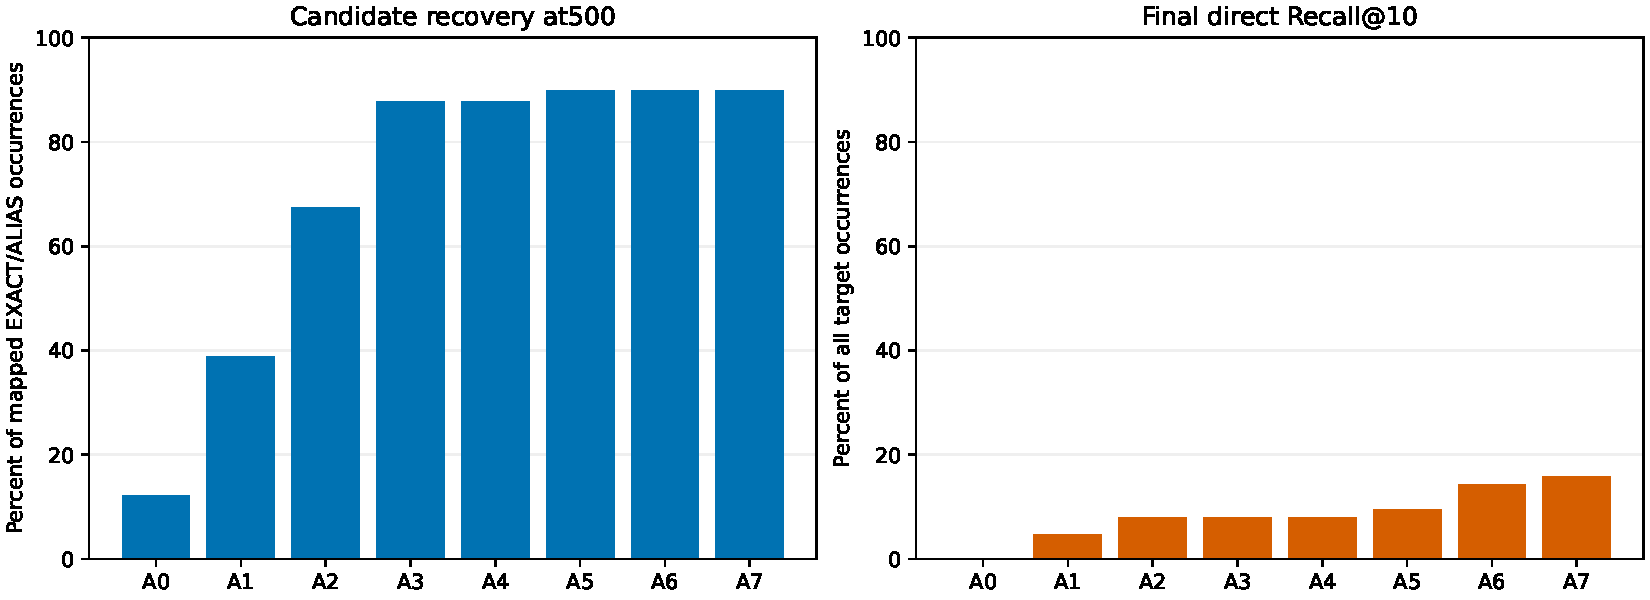
\includegraphics[width=\textwidth]{stage_metrics.pdf}
\caption{Two panels for the main stage sequence A0--A7. \emph{Left:} candidate recovery at depth 500, as a
percentage of the 49 mapped \texttt{EXACT}/\texttt{ALIAS} occurrences. \emph{Right:} final direct
$R@10$, as a percentage of all 63 target occurrences. The figure shows these two quantities only --- no
rank distributions and no additional cut-offs --- and the controls are not plotted. All values are
development diagnostics from the frozen artifacts.}
\label{fig:stage}
\end{figure}

\subsection{Candidate recall: hypothesis H1}
\label{sec:recall}

\begin{table}[htbp]
\centering
\small
\caption{Candidate pool recall. Hits are directly mapped target occurrences out of 49;
$R^{\text{cond}}$ is the /49 fraction and $R^{\text{raw}}$ the /63 fraction, both at depth 500. ``Union'' is
the full candidate pool regardless of depth. For the reranked arms the candidate pool is the
\emph{actual reranking prefix}: \texttt{A6\_100} and \texttt{A6\_200} cap their pools at 100 and 200 and are
saturated at greater depths, and A6/A7 cap at 500 (mean size 489.2 because some questions yield fewer than
500 eligible candidates). \textbf{No RRF tail is included in any candidate figure in this table}; the final
rankings of those arms do append the unchanged tail, which is why their observed-rank statistics in
Table~\ref{tab:ranks} cover 46 occurrences while their candidate pools contain 37--44.}
\label{tab:cand}
\resizebox{\textwidth}{!}{%
\begin{tabular}{lrrrrrrrrr}
\toprule
& \multicolumn{5}{c}{Hits at pool depth (/49)} & \multicolumn{2}{c}{Depth 500} & \multicolumn{2}{c}{Union} \\
\cmidrule(lr){2-6}\cmidrule(lr){7-8}\cmidrule(lr){9-10}
Arm & 50 & 100 & 200 & 500 & 1000 & $R^{\text{cond}}$ & $R^{\text{raw}}$ & hits & avg.\ size \\
\midrule
A0                      &  1 &  2 &  3 &  6 &  6 & 0.122 & 0.095 &  6 & 500.0 \\
A1                      &  5 & 10 & 16 & 19 & 19 & 0.388 & 0.302 & 19 & 489.2 \\
\texttt{TypedRaw}       &  5 & 10 & 16 & 19 & 19 & 0.388 & 0.302 & 19 & 489.2 \\
\texttt{ParsedOnly}     &  4 &  6 & 12 & 19 & 19 & 0.388 & 0.302 & 19 & 489.2 \\
A2                      & 11 & 20 & 24 & 33 & 43 & 0.673 & 0.524 & 43 & 913.6 \\
A3                      & 16 & 31 & 35 & 43 & 44 & 0.878 & 0.683 & 45 & 1108.9 \\
A4                      & 17 & 35 & 42 & 43 & 46 & 0.878 & 0.683 & 46 & 1295.6 \\
\textbf{A5}             & \textbf{29} & \textbf{37} & \textbf{43} & \textbf{44} & \textbf{46} & \textbf{0.898} & \textbf{0.698} & \textbf{46} & 1295.6 \\
\texttt{WithoutEvidenceRRF} & 17 & 29 & 40 & 45 & 46 & 0.918 & 0.714 & 46 & 1149.5 \\
\texttt{WithoutGraphRRF}    & 18 & 26 & 35 & 44 & 44 & 0.898 & 0.698 & 45 & 1108.9 \\
\texttt{A6\_100}        & 29 & 37 & 37 & 37 & 37 & 0.755 & 0.587 & 37 & 100.0 \\
\texttt{A6\_200}        & 29 & 37 & 43 & 43 & 43 & 0.878 & 0.683 & 43 & 200.0 \\
A6 ($=$\texttt{A6\_500}) & 29 & 37 & 43 & 44 & 44 & 0.898 & 0.698 & 44 & 489.2 \\
A7                      & 29 & 37 & 43 & 44 & 44 & 0.898 & 0.698 & 44 & 489.2 \\
\bottomrule
\end{tabular}}
\end{table}

Candidate set size ranges are 349--500 for A1/\texttt{TypedRaw}/\texttt{ParsedOnly}/A6/A7, 349--1090 for A2,
349--1324 for A3 and \texttt{WithoutGraphRRF}, 349--1503 for A4/A5, 349--1362 for
\texttt{WithoutEvidenceRRF}, and exactly 500, 100, 200 for A0, \texttt{A6\_100}, \texttt{A6\_200}.

On the recall question the observed development evidence is clear. A5 admits \textbf{37/49 at depth 100,
44/49 at depth 500, and 46/49 in the full union}, against \textbf{3/49 at depth 100} for the previous V2
high-recall arms and 2/49 for the previous V2 A0. The progression A1 $\to$ A2 $\to$ A3 $\to$ A4 shows that
most of the gain comes from channel addition rather than from fusion: depth-100 hits move 10 $\to$ 20 $\to$
31 $\to$ 35 under pure round-robin union. RRF then lifts depth-50 hits from 17 (A4) to 29 (A5) on the
identical union, which is the one place where ordering alone is demonstrably the operative mechanism.

\subsubsection*{Channel ablations}

Removing the evidence list from fusion drops A5's depth-50 hits from 29 to 17 and depth-100 from 37 to 29.
Removing the graph list drops the same figures to 18 and 26. Both lists matter at shallow depth and
\textbf{neither is categorically more important}: the evidence list is worth more at depth 50 (12 versus 11
occurrences) and the graph list is worth more at depth 100 (11 versus 8). Note also that
\texttt{WithoutEvidenceRRF} has the \emph{highest} depth-500 recall of any arm (45/49) while sharing A5's
union recall of 46/49, so that difference is a reordering effect inside the 500-prefix, not a loss of
coverage.

\begin{table}[htbp]
\centering
\small
\caption{Per-list diagnostics on the A4/A5 union. ``Unique'' = mapped occurrences recovered by that list and
no other.}
\label{tab:channel}
\begin{tabular}{lrrr}
\toprule
Ranked list & Mapped occurrences recovered & $R^{\text{cond}}$ (/49) & Unique \\
\midrule
Dense (original question)   & 19 & 0.388 & 0 \\
Dense (structured question) & 21 & 0.429 & 0 \\
BM25                        & 41 & 0.837 & 0 \\
Name                        &  0 & 0.000 & 0 \\
Evidence                    & 44 & 0.898 & 0 \\
Graph                       & 37 & 0.755 & 1 \\
\bottomrule
\end{tabular}
\end{table}

Table~\ref{tab:channel} is the most informative single diagnostic in the study. The name list recovers
\textbf{nothing}: these questions describe capabilities, not names, so exact-identity matching has no
opportunity. BM25 over the concatenated lexical document recovers 41/49 --- more than either dense view ---
so on this corpus the dense encoder, used without an instruction prefix and over bounded node renderings, is
weaker than term matching. The evidence list is the single strongest list at 44/49. Only the graph list
contributes anything \emph{uniquely} (one occurrence), so in terms of pure membership the lists are largely
redundant \emph{collectively}: nearly every occurrence found by the evidence list is also found by some other
list. That redundancy is about the union, not about ordering, and it is not the same as being useless at a
given depth: adding the evidence list to the round-robin union (A2 $\to$ A3, before graph was added) raised
depth-100 hits from 20 to 31. Membership redundancy with rank-level contribution is exactly the regime
Equation~\eqref{eq:rrf} is designed for.

\subsection{Final ranking metrics: hypothesis H2}
\label{sec:final}

\begin{table}[htbp]
\centering
\small
\caption{Final direct identity recovery. Hits are target occurrences out of 63; $R@k$ fractions use the
strict denominator 63. MRR denominator is 14.}
\label{tab:final}
\begin{tabular}{lrrrrrrr}
\toprule
& \multicolumn{6}{c}{Hits at rank $\le k$ (/63)} & \\
\cmidrule(lr){2-7}
Arm & 1 & 5 & 10 & 25 & 50 & 100 & MRR \\
\midrule
A0                          & 0 & 0 &  0 &  0 &  1 &  2 & 0.0044 \\
A1                          & 2 & 3 &  3 &  3 &  5 & 10 & 0.1666 \\
\texttt{TypedRaw}           & 2 & 3 &  3 &  3 &  5 & 10 & 0.1667 \\
\texttt{ParsedOnly}         & 0 & 2 &  3 &  3 &  4 &  6 & 0.0843 \\
A2                          & 2 & 3 &  5 &  6 & 11 & 20 & 0.1872 \\
A3                          & 2 & 4 &  5 & 10 & 16 & 31 & 0.1979 \\
A4                          & 2 & 4 &  5 & 10 & 17 & 35 & \textbf{0.2013} \\
A5                          & 0 & 4 &  6 & 11 & 29 & 37 & 0.1554 \\
\texttt{WithoutEvidenceRRF} & 0 & 3 &  3 &  8 & 17 & 29 & 0.1278 \\
\texttt{WithoutGraphRRF}    & 0 & 4 &  4 &  8 & 18 & 26 & 0.1374 \\
\texttt{A6\_100}            & 1 & 6 & \textbf{12} & 18 & 25 & 37 & 0.1669 \\
\texttt{A6\_200}            & 1 & 5 &  9 & 16 & 26 & 34 & 0.1523 \\
A6 ($=$\texttt{A6\_500})    & 1 & 5 &  9 & 14 & 22 & 33 & 0.1480 \\
\textbf{A7 (primary)}       & 1 & 5 & \textbf{10} & 14 & 22 & 33 & 0.1516 \\
\bottomrule
\end{tabular}
\end{table}

As fractions of 63, the declared primary A7 achieves $R@1 = 1.59\,\%$, $R@5 = 7.94\,\%$,
$R@10 = 15.87\,\%$, $R@25 = 22.22\,\%$, $R@50 = 34.92\,\%$, $R@100 = 52.38\,\%$. On the conditional /49
denominator the corresponding figures are $2.04\,\%$, $10.20\,\%$, $20.41\,\%$, $28.57\,\%$, $44.90\,\%$,
$67.35\,\%$.

Four observations:

\begin{enumerate}
\item \textbf{Top-10 recovery is higher than in the prior iterations.} A7 recovers 10/63 (15.87\,\%), against
3/63 for the previous V2's dense baseline arm, 2/63 for its relevance arm \texttt{V2-C}, 1/63 for
\texttt{V2-B}, and 0/63 for A0 in the matched re-run. This is the main evidence bearing on H2, and it
compares whole systems, not the cross-encoder in isolation.

\item \textbf{The best observed arm is a control.} \texttt{A6\_100} reaches 12/63 at top-10 and 18/63 at
top-25, above both A6 (9/63, 14/63) and A7 (10/63, 14/63), and it has the best conditional mean rank (77.70)
of the reranked arms. It does \emph{not} sweep every statistic: \texttt{A6\_200} has a marginally better
all-observed median (39.5 versus 40.0). The declared primary remains A7.

\item \textbf{No single ordering of the arms holds across metrics.} A4's round-robin union has the highest
MRR of any arm at 0.2013; RRF reordering lowers it to 0.1554 (A5), cross-encoder reranking to 0.1480 (A6),
and verification tiering recovers part of it at 0.1516 (A7), so MRR along the pipeline is non-monotonic.
Meanwhile A5 raises top-50 hits from 17 to 29 and loses both of A4's rank-1 hits ($R@1$: 2/63 $\to$ 0/63).
Whether A5 or A4 is ``better'' depends entirely on the operating depth, and no arm here is better on every
reported metric.

\item \textbf{Larger reranking pools were worse on top-10 in this run.} Top-10 hits fall 12 (pool 100), 9
(200), 9 (500), and the conditional median after reranking rises 27 $\to$ 38 $\to$ 50.5. The straightforward
reading is precision dilution: a bigger prefix gives the cross-encoder more opportunities to promote a
plausible-looking non-target above a target. This is an observed pattern over three pool sizes in one run,
not an established scaling law.
\end{enumerate}

\begin{table}[htbp]
\centering
\small
\caption{Observed-rank statistics over the final rankings. Mean and median are conditional on observed
direct ranks; the penalized mean assigns the fixed missing-rank penalty (5799) to each missing occurrence
and divides by 49.}
\label{tab:ranks}
\begin{tabular}{lrrrrr}
\toprule
Arm & median & mean & observed & missing & penalized mean \\
\midrule
A0                          & 208.0 & 220.00 &  6 & 43 & 5115.86 \\
A1                          &  97.0 & 118.68 & 19 & 30 & 3596.43 \\
\texttt{TypedRaw}           &  97.0 & 121.58 & 19 & 30 & 3597.55 \\
\texttt{ParsedOnly}         & 161.0 & 169.37 & 19 & 30 & 3616.08 \\
A2                          & 128.0 & 257.95 & 43 &  6 &  936.45 \\
A3                          &  70.0 & 159.18 & 45 &  4 &  619.57 \\
A4                          &  60.5 &  97.80 & 46 &  3 &  446.86 \\
A5                          &  39.5 &  80.85 & 46 &  3 &  430.94 \\
\texttt{WithoutEvidenceRRF} &  86.0 & 109.57 & 46 &  3 &  457.90 \\
\texttt{WithoutGraphRRF}    &  76.0 & 139.51 & 45 &  4 &  601.51 \\
\texttt{A6\_100}            &  40.0 &  77.70 & 46 &  3 &  427.98 \\
\texttt{A6\_200}            &  39.5 &  82.22 & 46 &  3 &  432.22 \\
A6 ($=$\texttt{A6\_500})    &  51.5 & 106.54 & 46 &  3 &  455.06 \\
A7                          &  51.5 & 106.24 & 46 &  3 &  454.78 \\
\bottomrule
\end{tabular}
\end{table}

Table~\ref{tab:ranks} shows why conditional statistics must be paired with miss counts. A0's conditional
mean rank of 220 looks respectable until one reads that it is computed over 6 observed occurrences with 43
missing; its penalized mean of 5115.86 is the honest summary. Conversely A2's conditional mean (257.95) is
\emph{worse} than A1's (118.68) while A2 observes 43 occurrences to A1's 19, and those extra 24 occurrences
sit deep in the list. The penalized means --- 936.45 for A2 against 3596.43 for A1 --- order the two the way
the recall figures do. Note that the reranked arms observe 46 occurrences here while their candidate pools
in Table~\ref{tab:cand} contain 37--44: the extra occurrences live in the appended, unreranked RRF tail.

\begin{table}[htbp]
\centering
\small
\caption{Previous V2 (archived) arms, same occurrence denominators. Candidate hits are out of 49. Rank
statistics there were computed over the full corpus, so misses are zero by construction.}
\label{tab:prev}
\begin{tabular}{lrrrrrr}
\toprule
Arm & $R@10$ hits & $R@100$ hits & MRR & median direct rank & cand.\ @100 & cand.\ @200 \\
\midrule
prev.\ A0  & 0 & 2 & 0.0047 & 3122 & 2 & 3 \\
prev.\ A1  & 3 & 6 & 0.1645 & 1293 & 6 & 8 \\
\texttt{V2-B} & 1 & 3 & 0.0168 & 1192 & 3 & 6 \\
\texttt{V2-C} & 2 & 3 & 0.0566 & 1192 & 3 & 6 \\
\bottomrule
\end{tabular}
\end{table}

These historical comparisons are \textbf{descriptive}. The hit counts and MRRs share the denominators used
here and are directly readable. The rank medians are not comparable to Table~\ref{tab:ranks}: the archived
arms ranked the whole corpus, so every target had a rank and the miss count was zero, whereas the new arms
truncate candidates and report conditional means with explicit misses. Both are internally valid; they
measure different things, and comparing them without the miss counts would be meaningless rather than
merely imprecise. The primary contrasts in this report are the \emph{matched new-run ablations} of
Tables~\ref{tab:cand} and~\ref{tab:final}, computed under identical denominators and identical candidate
caps.

\subsection{Conditional reranking analysis}
\label{sec:cond}

Conditional reranking statistics are computed only over target occurrences actually admitted to the
reranker's prefix; occurrences in the untouched tail cannot be moved and would dilute the measurement.

\begin{table}[htbp]
\centering
\small
\caption{Conditional reranking effects, restricted to target occurrences admitted to each prefix.
``New top-10'' counts occurrences that were outside top-10 before reranking and inside after.}
\label{tab:cond}
\begin{tabular}{lrrrrrrrr}
\toprule
Arm & pool & seen & up & down & median before & median after & top-10 after & new top-10 \\
\midrule
\texttt{A6\_100} & 100 & 37 & 17 & 20 & 36.0 & \textbf{27.0} & \textbf{12} & 7 \\
\texttt{A6\_200} & 200 & 43 & 19 & 24 & 39.0 & 38.0 & 9 & 5 \\
A6               & 500 & 44 & 18 & 26 & 39.0 & \textbf{50.5} & 9 & 5 \\
A7               & 500 & 44 & 18 & 26 & 39.0 & \textbf{50.5} & 10 & 6 \\
\bottomrule
\end{tabular}
\end{table}

At pool size 500, \textbf{of the 44 target occurrences seen by the reranker, 18 moved up and 26 moved down},
and the conditional median moved from 39 to 50.5. Conditional top-10 recall is 0.2273 for A7 and 0.2045 for
A6, against 0.3243 for \texttt{A6\_100}. So at pool 500 the cross-encoder lowered more target occurrences
than it raised while still placing more of them in the top 10 than fusion alone did: it concentrates a
handful of occurrences near the top and pushes the majority down. Both facts are measured and must be
reported together.

The verification tier (A7 versus A6) changes one occurrence's top-10 status and one question's first direct
rank in the frozen artifacts: in Q12, \texttt{DeePMD} moves from rank 20 to rank 7 and \texttt{GAP} from
rank 5 to rank 4, so Q12's first direct rank improves from 5 to 4 and A7 gains one top-10 occurrence (6 new
top-10 against 5 for A6). Every other per-question \emph{first} direct rank is identical between A6 and A7.
That is not the same as saying only one occurrence moved: tier reordering is applied to the whole top 20, so
other candidates --- including non-target entities and target occurrences that stayed outside the top 10 ---
may have changed position inside that window without changing any reported first-rank statistic. The
measured \emph{gain} attributable to the stage on this data is one top-10 occurrence, with MRR moving
0.1480 $\to$ 0.1516. The robustness of that gain is unmeasured: this is a single seeded run, no variance
estimate exists, and no hypothesis test was performed, so nothing here either establishes or excludes that a
rerun or a different question set would reproduce it.

\subsection{Selected strongest movements}

The following tables reproduce exact before/after ranks from the frozen handoff. They are presented as
\textbf{movements}, not explanations: the artifacts record ranks, not causes, and no causal attribution to
evidence similarity, card content or token truncation is inferred here. Rank movement also does not
adjudicate scientific relevance: an entity promoted above a target is not thereby shown to be a worse answer,
and a non-gold entity ranked highly is not thereby shown to be scientifically wrong.

\begin{table}[htbp]
\centering
\small
\caption{Strongest rank improvements and degradations under cross-encoder reranking at pool 500 (identical
for A6 and A7). Ranks are exact handoff values.}
\label{tab:mov500}
\begin{tabular}{llrr@{\qquad}llrr}
\toprule
\multicolumn{4}{c}{Improvements} & \multicolumn{4}{c}{Degradations} \\
\cmidrule(lr){1-4}\cmidrule(lr){5-8}
Q & Target & before & after & Q & Target & before & after \\
\midrule
Q9  & NequIP & 256 & 60 & Q12 & MACE                & 42 & 302 \\
Q13 & CGCNN  & 118 & 17 & Q12 & PET                 & 61 & 317 \\
Q13 & MACE   & 136 & 50 & Q7  & symbolic regression & 48 & 276 \\
Q13 & CHGNet & 113 & 35 & Q1  & ACE                 & 159 & 370 \\
Q10 & SchNet & 156 & 87 & Q4  & Hessian training    & 44 & 229 \\
\bottomrule
\end{tabular}
\end{table}

\begin{table}[htbp]
\centering
\small
\caption{Strongest rank improvements and degradations under cross-encoder reranking at pool 100
(\texttt{A6\_100}). Ranks are exact handoff values.}
\label{tab:mov100}
\begin{tabular}{llrr@{\qquad}llrr}
\toprule
\multicolumn{4}{c}{Improvements} & \multicolumn{4}{c}{Degradations} \\
\cmidrule(lr){1-4}\cmidrule(lr){5-8}
Q & Target & before & after & Q & Target & before & after \\
\midrule
Q12 & CHGNet       & 94 & 20 & Q12 & MACE & 42 & 86 \\
Q1  & CHGNet       & 72 & 15 & Q12 & eSEN & 12 & 53 \\
Q12 & DeePMD       & 62 &  8 & Q14 & WBM  & 29 & 68 \\
Q12 & GAP          & 50 &  4 & Q1  & MACE & 39 & 74 \\
Q12 & EquiformerV2 & 57 & 19 & Q12 & PET  & 61 & 89 \\
\bottomrule
\end{tabular}
\end{table}

Two patterns are worth recording. \texttt{MACE} is degraded in both Q1 and Q12 at every pool size (Q12:
$42 \to 86$ at pool 100, $42 \to 157$ at pool 200, $42 \to 302$ at pool 500), while \texttt{MACE} in Q13 is
\emph{improved} at pools 200 and 500 ($136 \to 40$ and $136 \to 50$). The same entity moves in opposite
directions for different questions, which is consistent with question-conditional scoring rather than a
per-entity bias. Separately, degradation magnitude grows with pool size for the same occurrence --- Q12
\texttt{PET} at $61 \to 89 \to 161 \to 317$ for pools 100/200/500 --- which is the occurrence-level counterpart
of the pool-size pattern in Table~\ref{tab:cond}.

\subsection{Per-question summary}

\begin{table}[htbp]
\centering
\small
\caption{Per-question first directly mapped rank. ``T'' = target occurrences; ``D'' = directly mappable
(\texttt{EXACT}/\texttt{ALIAS}) occurrences. ``--'' = no direct hit anywhere in the list.}
\label{tab:perq}
\begin{tabular}{lrrrrrrr}
\toprule
Q & T & D & A0 & A1 & A5 & A6 & A7 \\
\midrule
Q1  &  7 &  7 & --  & 193 &  23 &   3 &   3 \\
Q2  &  3 &  2 & 369 &  85 &   6 &  10 &  10 \\
Q3  &  2 &  1 &  57 &   1 &   2 &   7 &   7 \\
Q4  &  3 &  2 & --  &  37 &  33 &  69 &  69 \\
Q5  &  2 &  0 & --  & --  & --  & --  & --  \\
Q6  &  3 &  1 & 199 &   4 &   2 &  42 &  42 \\
Q7  &  2 &  1 & --  & --  &  48 & 276 & 276 \\
Q8  &  2 &  1 & --  & --  &   7 &   6 &   6 \\
Q9  &  3 &  1 & --  & --  & 256 &  60 &  60 \\
Q10 &  2 &  1 & --  & --  & 156 &  87 &  87 \\
Q11 &  2 &  0 & --  & --  & --  & --  & --  \\
Q12 & 13 & 13 &  31 &   1 &   2 &   5 &   4 \\
Q13 &  8 &  8 & --  & --  &  89 &  17 &  17 \\
Q14 & 11 & 11 & 217 &  26 &   4 &   1 &   1 \\
\midrule
Total & 63 & 49 & & & & & \\
\bottomrule
\end{tabular}
\end{table}

Q5 and Q11 have \textbf{no directly mappable target} and are structurally unanswerable under the direct
identity metric: Q5's targets are \texttt{Bead-mapping} (\texttt{ABSENT}) and \texttt{GNN+GPP}
(\texttt{PARTIAL}); Q11's are the \texttt{COMPOSITE} pipeline and \texttt{hybrid frameworks}
(\texttt{PARTIAL}). They contribute two guaranteed zeros to every arm's MRR, capping attainable MRR at
$12/14 = 0.857$ even with perfect rank-1 performance elsewhere.

At the first-hit level, reranking helps and hurts in comparable measure. Relative to A5, A6/A7 improve Q1
($23 \to 3$), Q8 ($7 \to 6$), Q9 ($256 \to 60$), Q10 ($156 \to 87$), Q13 ($89 \to 17$) and Q14 ($4 \to 1$),
and degrade Q2 ($6 \to 10$), Q3 ($2 \to 7$), Q4 ($33 \to 69$), Q6 ($2 \to 42$), Q7 ($48 \to 276$) and Q12
($2 \to 4$, or $2 \to 4$ for A7 after tiering). The Q6 case is the sharpest: \texttt{LiFlow} sits at rank 2
after fusion and falls to 42 after reranking.

\subsection{Failure analysis}
\label{sec:fail}

Every target occurrence receives one documented \textbf{primary} failure class at top-10, plus optional
secondary observations. The primary classes partition all 63 occurrences exactly.

\begin{table}[htbp]
\centering
\small
\caption{Primary failure classification at top-10 over all 63 target occurrences, and secondary
observations (non-exclusive). Codes are used in Appendix~\ref{app:ranks}.}
\label{tab:fail}
\begin{tabular}{llrp{7.0cm}}
\toprule
Code & Class & Count & Meaning \\
\midrule
CE  & \texttt{IN\_POOL\_CROSS\_ENCODER\_FAILED} & 34 & Occurrence was inside the 500-deep reranking prefix and is not in the final top 10. \\
R10 & \texttt{RECOVERED\_AT\_10} & 10 & Recovered at top-10 by the primary system. \\
GT  & \texttt{GROUND\_TRUTH\_MAPPING\_UNCERTAIN} & 14 & Non-direct annotation status (\texttt{PARTIAL}/\texttt{ABSENT}/\texttt{COMPOSITE}); no identity credit possible. \\
RRF & \texttt{IN\_POOL\_RRF\_FAILED} & 2 & In the union but ranked outside the 500-deep prefix by RRF, so never reranked. \\
TF  & \texttt{WRONG\_TYPE\_FILTER} & 3 & Excluded by the hard answer-family filter. \\
\midrule
    & Total & 63 & \\
\midrule
NN  & \texttt{NO\_NAME\_MATCH} (secondary) & 46 & No lexical opportunity: the question contains no surface form of the target. \\
NE  & \texttt{NO\_RELEVANT\_EVIDENCE} (secondary) & 8 & No indexed candidate-specific evidence existed. \\
\bottomrule
\end{tabular}
\end{table}

The largest class, \texttt{IN\_POOL\_CROSS\_ENCODER\_FAILED} at 34 of 63 occurrences, must be read exactly as
defined: these occurrences were \emph{inside the prefix and are not in the final top 10}. The class does
\textbf{not} mean 34 occurrences were actively demoted or lost by the cross-encoder; most of them were far
from the top 10 before reranking as well. The measured movement attributable to the reranker is the
conditional analysis of Table~\ref{tab:cond}: of the 44 admitted occurrences, 18 moved up and 26 moved down.
Nor does the small size of the fusion (2) and type-filter (3) classes license the conclusion that admission
has ceased to be a constraint --- five mapped occurrences never reached the reranker at all, including three
outside the union entirely, and 14 occurrences cannot be credited by
any system. What the distribution supports is narrower and still useful: at these depths, with this pool,
most remaining error is located after admission, in the ordering stages.

Concrete named traces, all from the frozen handoff:

\begin{itemize}
\item \textbf{Q13 \texttt{MEGNet}} and \textbf{Q13 \texttt{EquiformerV2}} are the two
\texttt{IN\_POOL\_RRF\_FAILED} cases, at ranks 733 and 551 respectively in A5, A6 and A7 alike. They are in
the union but beyond the 500-deep prefix, so their ranks are identical across all three arms by
construction: the tail is never touched.

\item \textbf{Q14 \texttt{JARVIS-DFT}}, \textbf{Q14 \texttt{AFLOW}} and \textbf{Q14 \texttt{Alexandria}} are
the three \texttt{WRONG\_TYPE\_FILTER} cases, with null ranks under every arm. Q14 requests ``datasets and
benchmarks'' ($\{\texttt{dataset}, \texttt{metric}\}$), and the graph nodes bearing these names are typed
outside those families, so Equation~\eqref{eq:allowed} removes them before retrieval. Three of Q14's eleven
occurrences are lost this way.

\item \textbf{Q12 \texttt{MACE}} is the largest single downward movement: rank 42 in A5, 302 in A6 and A7.
\textbf{Q12 \texttt{PET}} follows the same trajectory, 61 $\to$ 317; \textbf{Q7 \texttt{symbolic
regression}} 48 $\to$ 276; \textbf{Q1 \texttt{ACE}} 159 $\to$ 370.

\item \textbf{Q1 \texttt{GAP}} is a clean recovery: null in A0 and A1, rank 31 in A5, rank 3 in A6/A7.
\textbf{Q14 \texttt{Matbench Discovery}} moves 447 (A0) $\to$ 97 (A1) $\to$ 4 (A5) $\to$ 1 (A6/A7), and
\textbf{Q14 \texttt{Matbench}} 157 $\to$ 39 $\to$ 3. \textbf{Q8 \texttt{ConvLSTM}} is null in A0 and A1,
rank 7 in A5 and 6 in A6/A7 --- an occurrence the dense-only arms could not reach at all.

\item \textbf{Q12 \texttt{DeePMD}} is the occurrence whose top-10 status is attributable to the verification
stage: rank 62 in A5, 20 in A6, 7 in A7.

\item \textbf{Q2 \texttt{HamGNN}} (\texttt{PARTIAL}), \textbf{Q3 \texttt{xDeepH}} (\texttt{PARTIAL}),
\textbf{Q4 \texttt{MACE-F}} (\texttt{ABSENT}) and \textbf{Q11
\texttt{CE}$\rightarrow$\allowbreak\texttt{MC}$\rightarrow$\allowbreak\texttt{NN}$\rightarrow$\allowbreak\texttt{PF}} (\texttt{COMPOSITE})
illustrate the 14 \texttt{GROUND\_TRUTH\_MAPPING\_UNCERTAIN} occurrences: null under every arm by
annotation status rather than by retrieval behaviour.
\end{itemize}

Two terminological commitments. \texttt{NO\_RELEVANT\_EVIDENCE} means \emph{no indexed candidate-specific
evidence existed} --- an index coverage statement, not an adjudication that the entity is scientifically
irrelevant to the question. \texttt{NO\_NAME\_MATCH} means \emph{the absence of a lexical opportunity} ---
the question never names the target --- not that name matching was attempted and failed.

\subsection{Missing evidence versus contradiction}
\label{sec:verifres}

\begin{table}[htbp]
\centering
\caption{Requirement verification outcomes over the A7 top-20 candidates across all 18 questions.}
\label{tab:verif}
\begin{tabular}{lr}
\toprule
Quantity & Value \\
\midrule
Verification candidates ($18 \times 20$) & 360 \\
Requirement components evaluated & 800 \\
NLI inference pairs actually run & 376 \\
\quad of which \texttt{SUPPORTED} & 71 \\
\quad of which \texttt{CONTRADICTED} & 35 \\
\quad neutral / no clear result & 270 \\
Components with no eligible premise (inference skipped) & 424 \\
\texttt{NOT\_SUPPORTED\_BY\_AVAILABLE\_EVIDENCE} (total) & 694 \\
\bottomrule
\end{tabular}
\end{table}

Of 800 requirement components, only 376 had an eligible premise; the remaining 424 are
\texttt{NOT\_SUPPORTED\_BY\_AVAILABLE\_EVIDENCE} purely because the candidate-specific index, with
article-level and structural-path evidence excluded, contained nothing to score. Adding the 270 neutral NLI
outcomes gives the reported total of 694.

The status counts aggregate positive and exclusion components, whose polarities are opposite under
Equation~\eqref{eq:status}. The 71 \texttt{SUPPORTED} statuses therefore comprise positive components with
$P(\text{entail}) \ge 0.7$ and $P(\text{contra}) < 0.3$ \emph{together with} exclusion components with
$P(\text{contra}) \ge 0.7$ and $P(\text{entail}) < 0.3$; symmetrically for the 35 \texttt{CONTRADICTED}
statuses. Reading the aggregate as a single entailment-probability condition would be wrong unless exclusion
components happen to be absent, which the handoff does not report.

With that caveat, one distinction is substantive. \textbf{53\,\% of all components (424/800) are unsupported
for lack of a premise, not because anything contradicts them.} Only 35 components --- 4.4\,\% of the total,
9.3\,\% of actually inferred pairs --- show high proxy contradiction. A design that treated missing evidence
as contradiction would demote the majority of top-20 candidates on the basis of index sparsity rather than
evidence, and given that 2508 of 2978 entities have no candidate-specific evidence at all, that error would
systematically favour the well-documented entities.

Limitations of the NLI proxy:

\begin{itemize}
\item The probabilities are \textbf{uncalibrated}. The threshold $\tau = 0.7$ is a fixed design constant,
not a tuned or validated operating point, and no reliability diagram supports it.
\item \texttt{nli-deberta-v3-small} is a small general-domain model applied to materials-science claims far
outside its training distribution. It can misread quantitative conditions (``millions of atoms'',
``$>10^{3}$ atoms'', ``$\sim$50{,}000 compounds'') and it can misread negation and scope.
\item A premise is a single max-cosine evidence item, so verification is single-premise: a requirement
supported jointly by two pieces of evidence will not be recognised.
\item \textbf{This is not scientific entailment.} A \texttt{SUPPORTED} status means a small proxy model
assigned a high probability to one retrieved sentence under the polarity of Equation~\eqref{eq:status}; it is
not an adjudication that the method satisfies the requirement.
\item The measured gain of the whole stage on this data is one top-10 occurrence, with other movements inside
the top 20 not separately reported. Its robustness is unmeasured.
\end{itemize}

\subsection{Efficiency}

\begin{table}[htbp]
\centering
\small
\caption{Efficiency counters and descriptive timings. Counters are units of logical work, not target
occurrences. Timings are single-run CPU wall times.}
\label{tab:eff}
\begin{tabular}{lr}
\toprule
Quantity & Value \\
\midrule
Prediction phase wall time (s) & 865.24 \\
Query wall time (s) & 745.26 \\
Dense dot products & 295{,}920 \\
Evidence generation comparisons & 153{,}864 \\
BM25 document--term lookups (exact loop count) & 1{,}637{,}900 \\
Cross-encoder pairs & 8{,}849 \\
Cross-encoder actual inference pairs & 8{,}849 \\
Requirement evidence comparisons & 170{,}960 \\
Verification candidates & 360 \\
Verification components & 800 \\
NLI pairs & 376 \\
\midrule
Prefix timing estimate, pool 100 (s) & 170.12 \\
Prefix timing estimate, pool 200 (s) & 325.14 \\
Prefix timing estimate, pool 500 (s) & 675.01 \\
\bottomrule
\end{tabular}
\end{table}

All counters describe \textbf{logical work}, not production latency, and all timings are descriptive CPU wall
times on a single machine with 4 threads, batch size 32, seed 42.

Three caveats are material. First, the BM25 counter embedded in the predictor is a \emph{token-count
estimate}; the 1{,}637{,}900 figure is the document--term loop count implied by the frozen query intent and
the frozen tokenizer (entities $\times$ unique query terms, summed over questions), and it is the figure that
should be cited. Second, the prefix timing estimates for pools 100 and 200 are \textbf{amortized reuses of
the 500-run pair scores}: those controls never executed their own inference, so 170.12\,s and 325.14\,s are
reconstructions of what the measured 500-pool pairs imply, not observations. Third, cross-encoder pairs equal
actual inference pairs (8{,}849), confirming that no caching shortcut reduced the measured reranking workload
in the 500 run.

On these two axes together, \texttt{A6\_100} was both the best observed arm on top-10 recovery and the
cheapest reranking configuration, by roughly a factor of four in prefix time.

\section{Limitations}

\begin{enumerate}
\item \textbf{Development-only, design-exposed.} The questions and gold annotations were seen during V1
development, and that exposure motivated this work. Execution-time separation does not make this a held-out
result. Nothing here supports a publication claim or an inferential comparison.

\item \textbf{Scale.} 14 scored questions, 63 target occurrences, 49 directly mappable. One occurrence is
1.6 percentage points of $R@k$. The A7-versus-\texttt{A6\_100} top-10 gap is two occurrences.

\item \textbf{Annotation ceiling.} 14 of 63 occurrences (22\,\%) cannot receive identity credit under any
system, and two of 14 questions have no creditable target at all. Maximum attainable $R@k$ is
$49/63 = 77.8\,\%$; maximum attainable MRR is $12/14 = 0.857$.

\item \textbf{Index sparsity (schema coverage).} 2508 of 2978 entities have no candidate-specific evidence.
The evidence channel, the graph channel's evidence seeding, the cross-encoder card and the verification stage
are all structurally weaker for those entities. This is a coverage property of the graph. Those entities
remain reachable by the dense channels and by BM25 over names and aliases.

\item \textbf{Schema inference is structural.} Role arcs come from unique typed member signatures; ambiguous
\texttt{extends} arcs and signature mismatches are dropped rather than resolved, so some legitimate paths are
unavailable, and citation paths provide structural context and are never treated as entailment.

\item \textbf{Year-granular time filtering.} ``By Feb 2026'' is enforced at year granularity; month precision
is unrecoverable from year-only evidence. \texttt{first\_seen\_year} records publication visibility in this
graph, not an actual discovery date, and the undated-alias suppression rule only applies at cutoffs earlier
than a node's last observation.

\item \textbf{No calibration and no tuning.} Cross-encoder logits are not probabilities; NLI probabilities
are uncalibrated. Path decay (0.8), RRF $k$ (60), evidence/graph depths (500/200), family caps, the 512-token
budget and the NLI threshold (0.7) are fixed design constants; no hyperparameter search was performed, so
none is claimed optimal. The \texttt{soft\_type\_prior} key in \texttt{config.json} is legacy and unused.

\item \textbf{Controls beyond their prefix.} For \texttt{A6\_100} and \texttt{A6\_200}, final ranks beyond
the pool size come from the unchanged RRF tail, not from reranked entities, and their candidate figures in
Table~\ref{tab:cand} are capped at the pool. Comparing $R@100$ across pool sizes compares different objects
below the prefix boundary.

\item \textbf{Single run, no variance.} Every number is one seeded execution. No variance estimate and no
hypothesis test exists, so differences of one or two occurrences are reported as observations only.

\item \textbf{Ranks are not scientific adjudication.} The metrics score agreement with a small annotation
set. A high-ranked non-gold entity is not shown to be a wrong answer, and a low-ranked gold entity is not
shown to be irrelevant.

\item \textbf{Historical comparisons are descriptive.} Prior V1 and V2 figures were computed under different
candidate truncation and grouping conventions; their rank statistics are not commensurate with the
conditional statistics here.
\end{enumerate}

\section{Future work}

Two questions are open, and neither can be settled by rerunning arms that already exist in this study.
\texttt{A6\_100} is such an arm: it is reported above as a predeclared control, so a ``cascade that reranks
only the top 100'' is a configuration already measured here, not a new experiment, and quoting its 12/63 as
a prediction would be reporting a known result.

\begin{enumerate}
\item \textbf{Pool choice needs independent data.} The pool-size pattern (top-10 hits 12/9/9; conditional
median 27/38/50.5) comes from the same 14 design-exposed questions used to build the system. The appropriate
next step is to assemble an \emph{independent} question and target set --- new questions, annotated without
reference to this system's outputs --- and to register the pool-size comparison on that set before running
it. Until then the pool choice is a development observation.
\item \textbf{Evidence packing is a hypothesis, not a finding.} The large downward movements (Q12
\texttt{MACE} $42 \to 302$, Q12 \texttt{PET} $61 \to 317$) have exported card contents: included blocks,
omitted blocks and token counts are already in the frozen artifacts. The honest sequence is to
\emph{inspect those existing traces first}, descriptively, and only then preregister a comparison of
alternative evidence-packing policies --- different family caps, different block order, best-fit instead of
prefix packing --- on new data. No such comparison is predeclared here, and no tuning of packing on the
present benchmark should be presented as a held-out result afterwards.
\end{enumerate}

Nothing in the present data justifies extending the verification stage; its measured gain is one occurrence
and should be held fixed while the questions above are addressed. The three \texttt{WRONG\_TYPE\_FILTER}
occurrences are a separate, concrete item: widening Q14-style coordinated answer families would be a design
change whose cost in admitted noise is currently unmeasured.

\section{Reproducibility}

\begin{table}[htbp]
\centering
\small
\caption{Pinned model versions. All models are loaded locally from hashed caches; downloads require an
explicit \texttt{--download} flag. Revisions wrap across lines and concatenate to the exact literal value.}
\label{tab:models}
\begin{tabular}{p{2.3cm}p{4.1cm}p{5.2cm}l}
\toprule
Role & Model & Revision & Status \\
\midrule
Dense & \texttt{BAAI/bge-small-en-v1.5} & \hx{5c38ec7c405ec4b44b94}{cc5a9bb96e735b38267a} & available \\
Relevance & \texttt{cross-encoder/\allowbreak ms-marco-MiniLM-L6-v2} & \hx{233902d25c440f23af6f}{7d6e94d2946bac0bee0a} & available \\
NLI (verification only) & \texttt{cross-encoder/\allowbreak nli-deberta-v3-small} & \hx{fa2804872c3b4bd748f3}{8c0185cc85775361e735} & available \\
\bottomrule
\end{tabular}
\end{table}

The following links identify the pinned local artifacts only; no external source was consulted for this
report: \url{https://huggingface.co/BAAI/bge-small-en-v1.5},
\url{https://huggingface.co/cross-encoder/ms-marco-MiniLM-L6-v2},
\url{https://huggingface.co/cross-encoder/nli-deberta-v3-small}.

Environment: Python 3.11.2 (MSC v.1934, 64-bit), CPU device, seed 42, 4 threads, batch size 32;
\texttt{numpy} 2.3.5, \texttt{torch} 2.4.1, \texttt{transformers} 4.57.6,
\texttt{sentence-transformers} 5.1.0, \texttt{huggingface-hub} 0.36.2. No model load failures were recorded.
All per-file SHA256 digests for the three model caches are recorded in
\path{outputs/audit/model_version_manifest.json}.

\subsection{Two distinct determinism checks}

These are different checks with different scopes and are not interchangeable:

\begin{enumerate}
\item \textbf{Replay check.} The replay reuses \emph{cached model outputs} and verifies that the full
prediction byte stream reproduces identically against the frozen digest \\
\hx{5bc46c27e260572cc33630ff59b3dd14}{2cc37ca5ef66d13eb77f29b1a2ad0eda}. \\
This establishes byte-identical replay of the deterministic pipeline logic --- grouping, filtering, union
construction, RRF ordering, tie-breaking, card packing, tier assignment, serialization --- \emph{given the
cached model outputs}. It does not re-execute the neural models and therefore says nothing about
reproducibility of an uncached full-model run.
\item \textbf{Fixed-input model determinism tests.} Separate synthetic tests feed fixed inputs to the pinned
\emph{dense encoder} and the pinned \emph{relevance cross-encoder} and check that the inference output is
bit-stable, with deterministic algorithms enabled, when those models are available. The \textbf{NLI
verification model is not covered} by this check; the NLI model is covered only by the status-semantics and
policy tests, which assert that it is never used as a relevance scorer.
\end{enumerate}

Together they establish deterministic pipeline logic given cached outputs, and bit-stable inference for two
of the three models given identical inputs. Neither establishes --- nor is claimed to establish ---
stability across hardware, library versions, uncached reruns, or re-trained checkpoints.

\subsection{Scope of the change}

The active implementation is \texttt{clean\_tshc\_v2}. The previous V2 source, config, report and results are
archived under \path{archive/flat_20261001}. The experiment does \textbf{not} route through the hierarchy
component and does not place it on any critical path.

Regarding V1: at the start of this work, V1 already contained two pre-existing uncommitted tracked report
changes and four untracked report files, and the user explicitly approved \textbf{preserving that starting
state}. The commitment made and kept is therefore that \textbf{this work introduces zero additional changes
to V1} --- not that \texttt{git diff} in V1 is empty. V1 hashes and diff should be compared against that
approved starting state, not against \texttt{HEAD}. No GitHub operations of any kind were performed.

\subsection{Verification and test tallies}

Digest verification and the automated test suite are executed by Codex; the audited tallies are reproduced
here. The test run observed at the time of writing was 42 tests passing in 16.35\,s.

\IfFileExists{verification_summary.tex}{\subsection*{Final verification by Codex}
The complete V2 suite passed: \textbf{42 tests passed in 16.35 seconds}, including existing regression tests and the new entity-pipeline and frozen-artifact checks. Prediction/source/input hashes verify, and the full cached replay has the same prediction SHA256. The positive and empty-ranking evaluation controls pass. V1 has \textbf{zero new modifications}: all 1,056 file hashes, the binary git diff, and V1 git-status entries match the user-approved starting state. Existing V1 report changes were preserved. No GitHub changes were made.
The machine-readable verification, changed/added-file inventory, and final artifact hashes are under \path{outputs/audit/}. These checks do not turn development diagnostics into held-out evidence.
}{}

\section{AI contribution disclosure}

\begin{itemize}
\item \textbf{Codex} implemented the pipeline, integrated all components, executed the experiment, produced
every measurement, supplied the factual corrections incorporated into this revision, and performs the
numerical verification, digest checks, test runs and compilation of this report.
\item \textbf{Claude Opus 5} supplied a methodology consultation --- on metric denominators, failure
classification, leakage ordering and the separation of the two determinism checks --- authored this report
from the frozen measured artifacts (\path{notes/entity_redesign/method_specification.md},
\path{notes/entity_redesign/report_handoff.json}, \path{config.json},
\path{outputs/audit/model_version_manifest.json} and the pipeline source), and revised it against Codex's
corrections. Claude did not run the experiment, did not produce any measurement, and did not select which
arm is primary.
\end{itemize}

\textbf{This report is not human expert adjudication and not a held-out publication result.} It is a
development diagnostic produced by AI agents from frozen artifacts, over a question set that was visible
during earlier design iterations, at a scale (14 questions, 63 target occurrences) where single-occurrence
differences dominate the reported margins. The declared primary system is A7, as predeclared, and is
reported as such even though a predeclared control performs better on the headline metric.

\appendix
\section{Full question texts}

\begin{longtable}{p{0.8cm}p{14.2cm}}
\toprule
ID & Question (verbatim) \\
\midrule
\endfirsthead
\toprule
ID & Question (verbatim) \\
\midrule
\endhead
\bottomrule
\endfoot
Q1 & Which methods (by Feb 2026) are best suited for predicting interatomic potentials when balancing accuracy close to DFT with computational efficiency for systems of millions of atoms? \\
Q2 & Which methods (by Feb 2026) are best suited for accelerating electronic structure calculations when self-consistent field iterations become prohibitively expensive for large systems ($>10^{3}$ atoms)? \\
Q3 & Which methods (by Feb 2026) are best suited for learning DFT Hamiltonians when dealing with twisted van der Waals heterostructures containing thousands of magnetic atoms? \\
Q4 & Which methods (by Feb 2026) are best suited for phonon property prediction when universal MLIPs show inaccuracies despite good energy/force performance? \\
Q5 & Which methods (by Feb 2026) are best suited for coarse-graining molecular dynamics when crystalline symmetries and long-range elastic interactions must be preserved? \\
Q6 & Which methods (by Feb 2026) are best suited for predicting ionic conductivity when full ab initio MD is too expensive but accuracy must be maintained? \\
Q7 & Which methods (by Feb 2026) are best suited for predicting phase transitions when screening $\sim$50,000 inorganic compounds at high throughput? \\
Q8 & Which methods (by Feb 2026) are best suited for predicting fracture patterns when generalizing from atomistic MD data to unseen bicrystalline structures? \\
Q9 & Which methods (by Feb 2026) are best suited for ensuring physical consistency when transferring information between scales without violating thermodynamic principles? \\
Q10 & Which methods (by Feb 2026) are best suited for representing atomic environments when the system exhibits significant compositional diversity, defects, and disorder? \\
Q11 & Which methods (by Feb 2026) are best suited for integrating features from three or more distinct scales simultaneously within a unified framework? \\
Q12 & What are the leading (by Feb 2026) ML-based interatomic potential methods for large-scale atomistic simulation? \\
Q13 & What are the leading (by Feb 2026) GNN architectures for predicting properties of solid-state crystalline materials? \\
Q14 & What datasets and benchmarks are commonly used (by Feb 2026) to evaluate MLIPs and property prediction models for materials discovery? \\
\end{longtable}

\section{Per-occurrence target ranks}
\label{app:ranks}

Annotation statuses: E $=$ \texttt{EXACT}, A $=$ \texttt{ALIAS}, P $=$ \texttt{PARTIAL},
X $=$ \texttt{ABSENT}, C $=$ \texttt{COMPOSITE}. Failure codes are those of Table~\ref{tab:fail}:
CE, R10, GT, RRF, TF. ``--'' $=$ not retrieved by that arm.

\begin{longtable}{p{0.7cm}p{3.9cm}p{0.5cm}rrrrrp{0.85cm}}
\toprule
Q & Target & St & A0 & A1 & A5 & A6 & A7 & Fail \\
\midrule
\endfirsthead
\toprule
Q & Target & St & A0 & A1 & A5 & A6 & A7 & Fail \\
\midrule
\endhead
\bottomrule
\endfoot
Q1 & MACE & E & -- & -- & 39 & 174 & 174 & CE \\
Q1 & M3GNet & E & -- & 193 & 35 & 51 & 51 & CE \\
Q1 & CHGNet & E & -- & 309 & 72 & 31 & 31 & CE \\
Q1 & GAP & E & -- & -- & 31 & 3 & 3 & R10 \\
Q1 & NequIP & E & -- & 354 & 24 & 56 & 56 & CE \\
Q1 & ACE & E & -- & -- & 159 & 370 & 370 & CE \\
Q1 & EquiformerV2 & E & -- & -- & 23 & 54 & 54 & CE \\
Q2 & DeepH & E & -- & -- & 40 & 15 & 15 & CE \\
Q2 & D4FT & E & 369 & 85 & 6 & 10 & 10 & R10 \\
Q2 & HamGNN & P & -- & -- & -- & -- & -- & GT \\
Q3 & xDeepH & P & -- & -- & -- & -- & -- & GT \\
Q3 & DeepH-E3 & E & 57 & 1 & 2 & 7 & 7 & R10 \\
Q4 & Hessian training & A & -- & 37 & 44 & 229 & 229 & CE \\
Q4 & VGNN & E & -- & -- & 33 & 69 & 69 & CE \\
Q4 & MACE-F & X & -- & -- & -- & -- & -- & GT \\
Q5 & Bead-mapping & X & -- & -- & -- & -- & -- & GT \\
Q5 & GNN+GPP & P & -- & -- & -- & -- & -- & GT \\
Q6 & DeePMD+AL & P & -- & -- & -- & -- & -- & GT \\
Q6 & LiFlow & E & 199 & 4 & 2 & 42 & 42 & CE \\
Q6 & MLIP descriptors & P & -- & -- & -- & -- & -- & GT \\
Q7 & GNN free energies & P & -- & -- & -- & -- & -- & GT \\
Q7 & symbolic regression & E & -- & -- & 48 & 276 & 276 & CE \\
Q8 & ConvLSTM & E & -- & -- & 7 & 6 & 6 & R10 \\
Q8 & GNN stress fields & P & -- & -- & -- & -- & -- & GT \\
Q9 & E(3)-equivariant GNNs & P & -- & -- & -- & -- & -- & GT \\
Q9 & physics-informed & P & -- & -- & -- & -- & -- & GT \\
Q9 & NequIP & E & -- & -- & 256 & 60 & 60 & CE \\
Q10 & GNNs $+$ ACE descriptors & P & -- & -- & -- & -- & -- & GT \\
Q10 & SchNet & E & -- & -- & 156 & 87 & 87 & CE \\
Q11 & CE$\rightarrow$MC$\rightarrow$NN$\rightarrow$PF & C & -- & -- & -- & -- & -- & GT \\
Q11 & hybrid frameworks & P & -- & -- & -- & -- & -- & GT \\
Q12 & MACE & E & -- & -- & 42 & 302 & 302 & CE \\
Q12 & NequIP & E & -- & -- & 39 & 65 & 65 & CE \\
Q12 & CHGNet & E & -- & 252 & 94 & 38 & 38 & CE \\
Q12 & M3GNet & E & -- & 141 & 36 & 108 & 108 & CE \\
Q12 & SevenNet & E & -- & -- & 40 & 50 & 50 & CE \\
Q12 & GAP & E & -- & -- & 50 & 5 & 4 & R10 \\
Q12 & DeePMD & E & -- & -- & 62 & 20 & 7 & R10 \\
Q12 & MatterSim & E & 31 & 1 & 2 & 24 & 24 & CE \\
Q12 & Orb & E & -- & -- & 26 & 52 & 52 & CE \\
Q12 & eSEN & E & -- & 97 & 12 & 99 & 99 & CE \\
Q12 & PET & E & -- & -- & 61 & 317 & 317 & CE \\
Q12 & UMA & E & -- & -- & 67 & 161 & 161 & CE \\
Q12 & EquiformerV2 & E & -- & -- & 57 & 37 & 37 & CE \\
Q13 & CGCNN & E & -- & -- & 118 & 17 & 17 & CE \\
Q13 & SchNet & E & -- & -- & 115 & 198 & 198 & CE \\
Q13 & MEGNet & E & -- & -- & 733 & 733 & 733 & RRF \\
Q13 & M3GNet & E & -- & -- & 95 & 142 & 142 & CE \\
Q13 & NequIP & E & -- & -- & 89 & 121 & 121 & CE \\
Q13 & MACE & E & -- & -- & 136 & 50 & 50 & CE \\
Q13 & CHGNet & E & -- & -- & 113 & 35 & 35 & CE \\
Q13 & EquiformerV2 & E & -- & -- & 551 & 551 & 551 & RRF \\
Q14 & Matbench Discovery & E & 447 & 97 & 4 & 1 & 1 & R10 \\
Q14 & Matbench & E & -- & 157 & 39 & 3 & 3 & R10 \\
Q14 & JARVIS-DFT & E & -- & -- & -- & -- & -- & TF \\
Q14 & Materials Project & E & -- & 75 & 15 & 49 & 49 & CE \\
Q14 & MPtrj & E & -- & 108 & 37 & 16 & 16 & CE \\
Q14 & OQMD & E & -- & 120 & 33 & 67 & 67 & CE \\
Q14 & AFLOW & E & -- & -- & -- & -- & -- & TF \\
Q14 & Alexandria & E & -- & -- & -- & -- & -- & TF \\
Q14 & GNoME & E & -- & 69 & 26 & 10 & 10 & R10 \\
Q14 & WBM & E & 217 & 26 & 29 & 86 & 86 & CE \\
Q14 & OMat24 & E & -- & 129 & 21 & 4 & 4 & R10 \\
\end{longtable}

\section{Fixed configuration constants}

Snapshot 2026; seed 42; 4 threads; batch size 32. Channel depth 500 per list; RRF $k = 60$; BM25
$k_1 = 1.5$, $b = 0.75$; evidence seed depth 500; graph seed depth 200, article degree cap 80, fanout cap
64, max 2 hops, path decay 0.8; rerank prefix 500 with controls at 100 and 200; cross-encoder token budget
512; card family caps claims 4, explicit mentions 3, tasks 2, problems 2, techniques 2, components 2,
datasets 1, metrics 1, articles 1, graph evidence 2; verification $k = 20$; NLI threshold 0.7; verification
policy \texttt{stable\_top20\_tiers\_all\_supported\_then\_unresolved\_then\_contradicted}; diffusion arm not
run. The key \texttt{soft\_type\_prior} $= 0.8$ is present in \path{config.json} but unused by this
pipeline.

\end{document}
